\section{Malleable TOHTN Planning}
- upgrade from moldable to malleable task according to \cite{feitelson1997job} as introduced in section \ref{prelim: malleability}
- we can no longer assume that messages always arrive and get a response
- we want to achieve completeness
- when sending a message, we always want to send it to another 

\subsection{Adapting CrowdHTN to a Malleable Environment}
As discussed in section \ref{prelim: crowdhtn}, CrowdHTN in its original form is a moldable program, with the number of parallel workers fixed for each single execution. To adapt CrowdHTN to work as a malleable program within Mallob, we have to address three key concerns.
\begin{enumerate}
	\item Messages sent to workers who are suspended or terminated before it arrives
	\item Integrating new processes to work efficiently
	\item Dealing with workers dying without loosing completeness
\end{enumerate}
To help understanding, this section explicitly discerns between Mallob workers and Crowd workers. \todo{more terminology}
\paragraph{Messages sent to dead workers}
As Mallob runs each worker in a different processes communicating via message passing, we never have a full view of the current global state of our process, i.e., which other Mallob workers are assigned to the same job. Instead we only ever get information about this that might be outdated. As a result, when a message such as a work request is sent to another worker, we cannot be sure that the receiving worker is in a position to actually respond. Luckily, Mallob does provide us with a mechanism to detect such messages. Each Mallob worker knows which job it currently works on and all messages are tagged with their job as well. If a message belonging to job $J_i$ is received by a worker working on job $J_k, k \neq i$, the message is simply tagged with a \textit{returned to sender} flag and sent back. \\
Now we can simply adapt CrowdHTN to deal with each message both if it is received normally and if it is received as a return message. On normal messages, nothing changes. On return messages we do the following:
\begin{itemize}
	\item \textbf{Work request}: we treat this like a negative response. This means we set the \textit{has active work request} flag to false and simply send out another work request at the next chance.
	\item \textbf{Positive work response}: this is the node we sent out ourselves. As to not loose any information, we simply re-insert the node at the front of our local fringe. While this may slightly change the order of the nodes at the front, we expect the number of outgoing work packages at any point to be small and the disturbance to be limited. In case of random searches, it should not negatively affect our algorithm.
	\item \textbf{Negative work response}: we do not have to care about this and can simply ignore it.
	\item \textbf{Ack}: we do not have to care about this and can simply ignore it.
\end{itemize}
While this mechanism should deal with most cases of workers dying, we can always construct pathological cases in which the return message mechanism fails. One such exchange can be seen in graphic \ref{malleable: lost message}. One way of dealing with this would be to change the way Mallob handles messages whose receiver is no longer valid. E.g., if a return message was delivered to a worker who changed jobs in the meantime, one could instead find out the root worker of the accompanying job and send the message there instead.
\todo{ref that the root always lives at least as long as everything else}
This way no information would be lost until we decide to terminate the whole job at which point this would be unavoidable and okay by the user. To avoid having to change Mallob, we instead elected to make our adaptation of CrowdHTN resistant to such information loss.
\todo{write about loop detection and restarts here}
\begin{figure}
	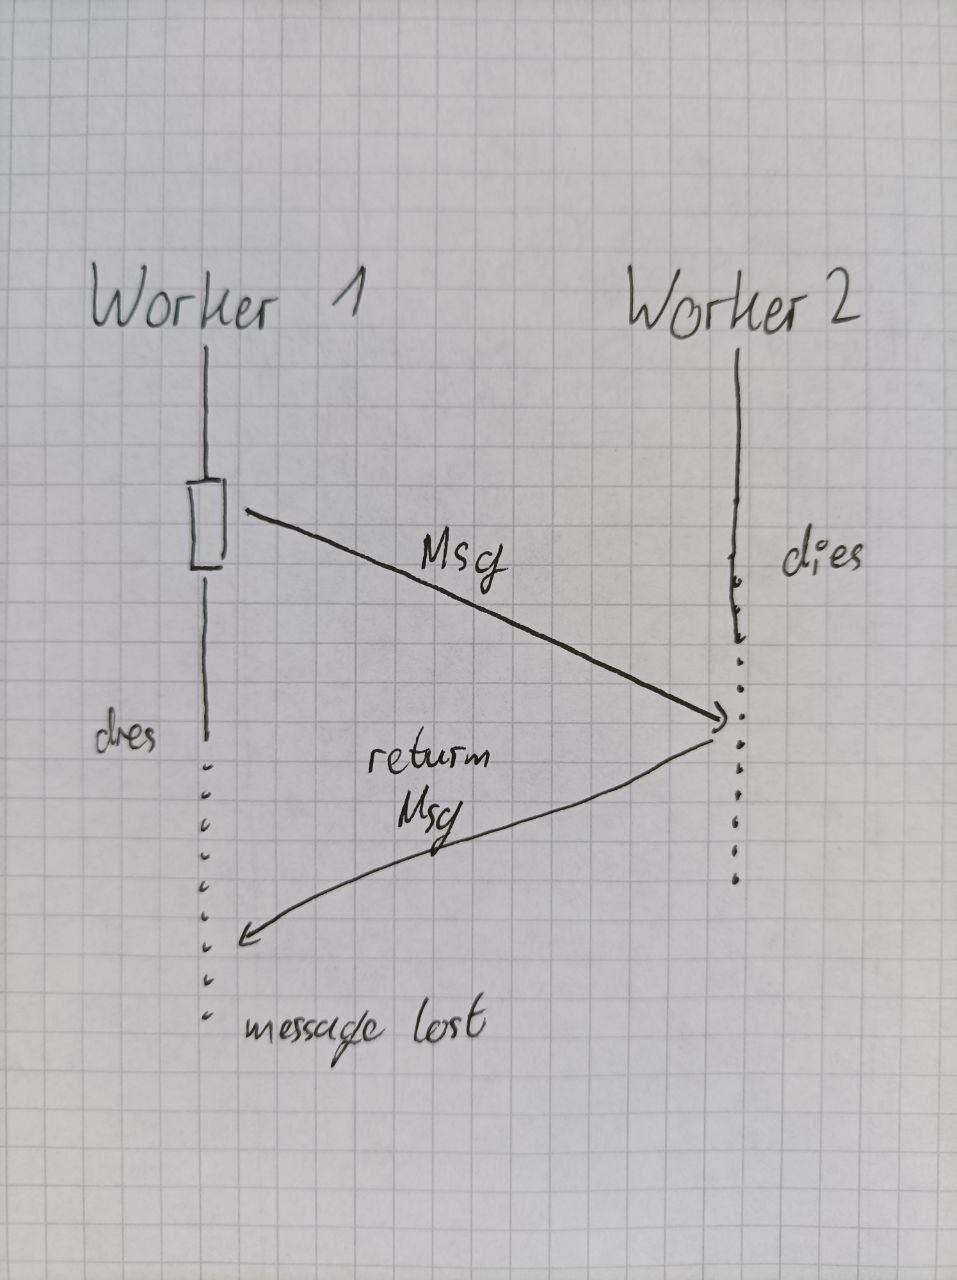
\includegraphics[width=0.6\textwidth]{images/prelim/malleable_lost_message}
	\caption{Example diagram of a lost message}
	\label{malleable: lost message}
\end{figure}

\paragraph{Integrating new workers}
As CrowdHTN uses work stealing to distribute work and perform load balancing, new workers can be seamlessly integrated into a running job. Upon construction all workers are treated the same, whether they are part of the initial batch or appear at a later point. The root worker is initialized with the initial search node, all other nodes are empty. To get new work, a worker sends a work request to a random other node and then goes from there. The very same process can be used to integrate a new worker.

\paragraph{Dealing with the information loss of dying workers}
- possible ways:
	- send back the root, delete from the loop detection -> most feasible, still looses a lot
	- send back the current fringe -> too much communication
	- ignore, do it with restarts -> easiest, we want restarts anyways. Has the consequence of loosing the UNPLAN capability as running out of work may simply be due to information loss induced by dying workers

- how to deal with workers leaving
	- hard, what if the parent is dead, too?
	- same as missing messages

- ensure completeness
- ensure performance
- work stealing is kinda nice here
